\documentclass[10pt]{article}
\usepackage{longtable}
\usepackage{float}
\usepackage{wrapfig}
\usepackage{rotating}
\usepackage[normalem]{ulem}
\usepackage{amsmath}
\usepackage{textcomp}
\usepackage{marvosym}
\usepackage{wasysym}
\usepackage{amssymb}
\usepackage{hyperref}
\usepackage{color,soul} % for highlighting
\usepackage{graphicx}
\graphicspath{{/Users/benjaminbass/seacloud/class/earthMaterials/picBank/}}

\usepackage{frame,color}
\usepackage{framed}
\usepackage{minibox}

% \usepackage[T1]{fontenc}
% \usepackage{tilting} %bring title up
% \setlength{\droptitle}{-10cm}

\usepackage[version=3]{mhchem}
% How to Use MChem
% \ce{SO4^2-}
% \ce{^{227}_{90}Th+}
% \ce{A\bond{-}B\bond{=}C\bond{#}D}
% \ce{CO2 + C -> 2CO}
% \ce{SO4^2- + Ba^2+ -> BaSO4 v}


\author{Benjamin Bass}
\date{15 March 2016}
\title{\vspace{-2.0cm}  Andalusite} %bring title up temporary Fix

\begin{document}

\maketitle

% \framebox{Use frameboxes until figure out alignmen}

\begin{center}
  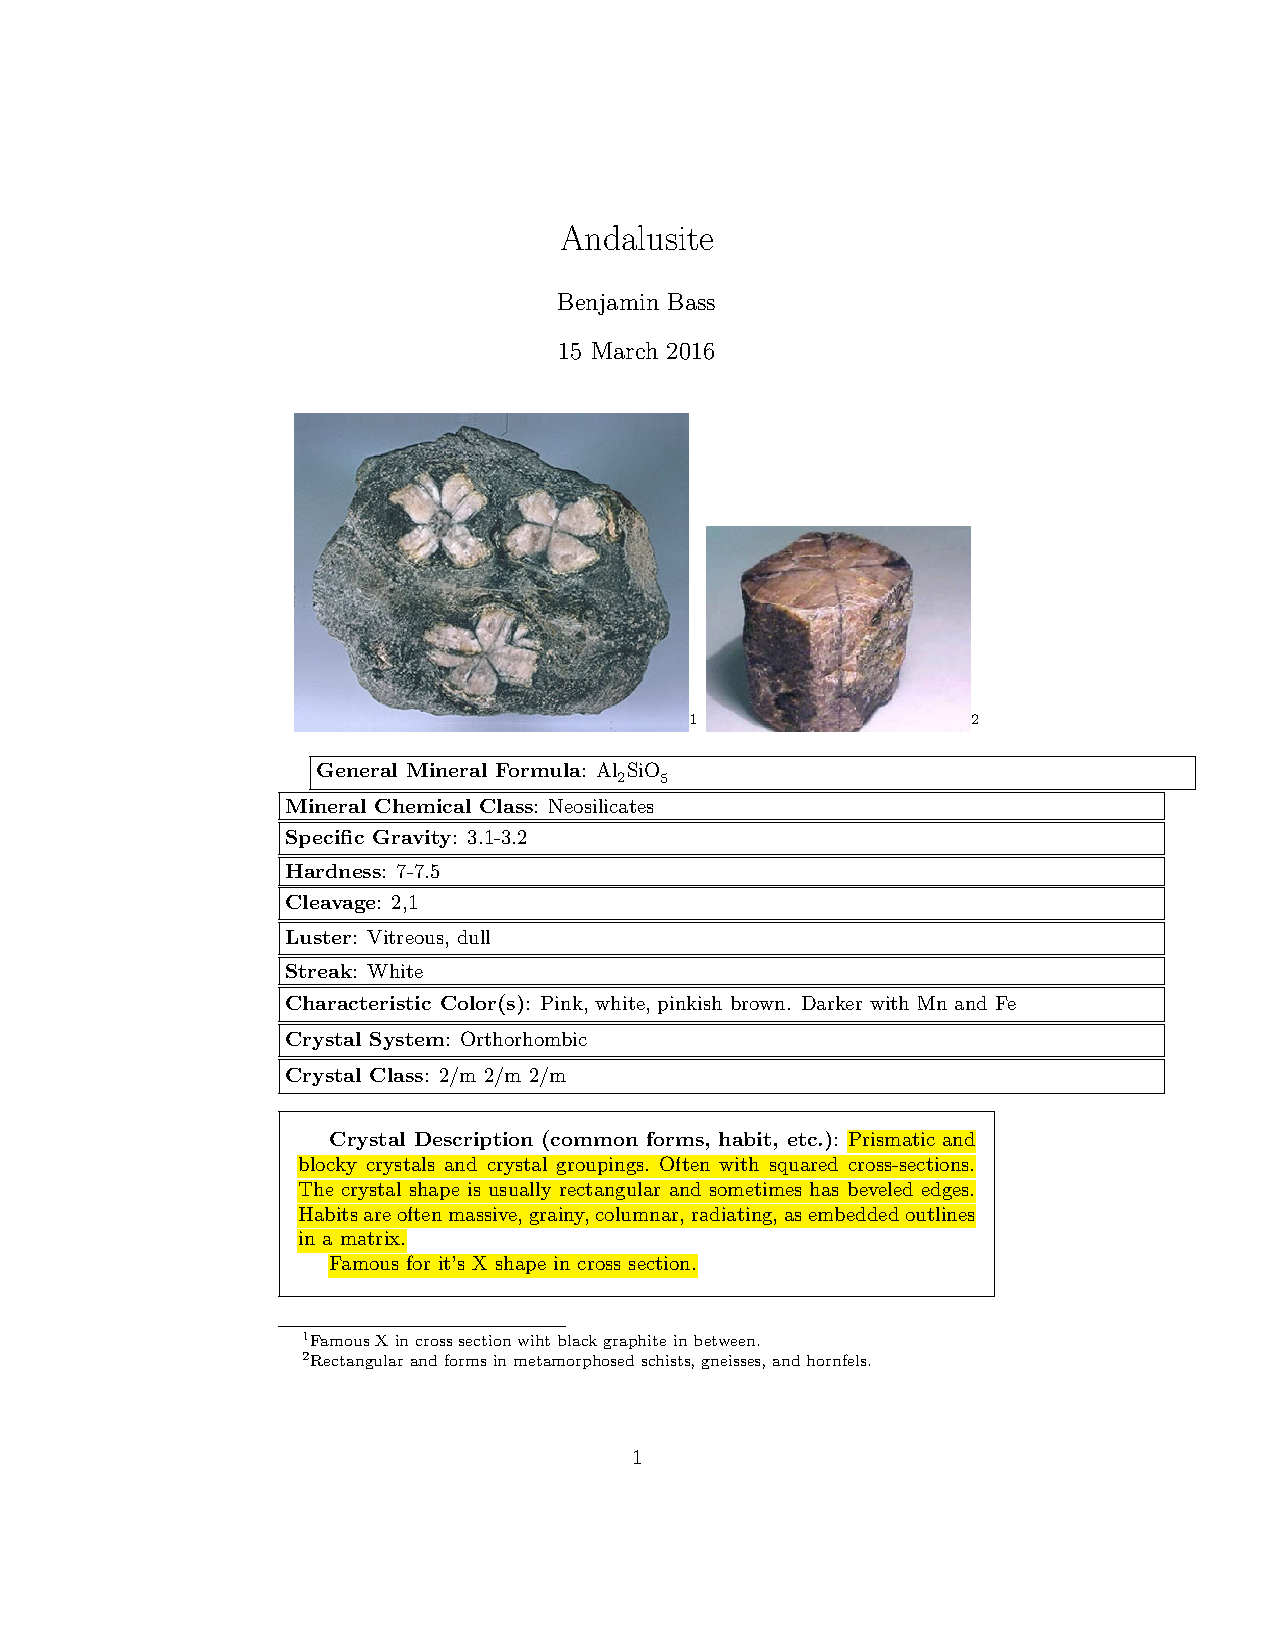
\includegraphics[scale=0.5]{andalusite}\footnote{Famous X in cross section wiht black graphite in between.}
  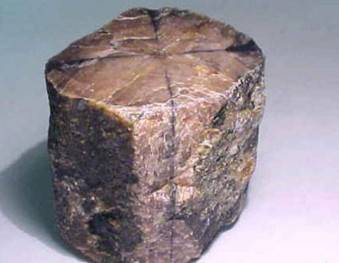
\includegraphics[scale=0.5]{andalusite2}\footnote{Rectangular and forms in metamorphosed schists, gneisses, and hornfels.}
\end{center}



\framebox[15cm][l]{\textbf{General Mineral Formula}: \ce{Al2SiO5} }\
\framebox[15cm][l]{\textbf{Mineral Chemical Class}: Neosilicates }\
\framebox[15cm][l]{\textbf{Specific Gravity}: 3.1-3.2 }\
\framebox[15cm][l]{\textbf{Hardness}: 7-7.5 }\
\framebox[15cm][l]{\textbf{Cleavage}: 2,1 }\
\framebox[15cm][l]{\textbf{Luster}: Vitreous, dull }\
\framebox[15cm][l]{\textbf{Streak}: White }\
\framebox[15cm][l]{\textbf{Characteristic Color(s)}: Pink, white, pinkish brown. Darker with Mn and Fe }\
\framebox[15cm][l]{\textbf{Crystal System}: Orthorhombic }\
\framebox[15cm][l]{\textbf{Crystal Class}: 2/m 2/m 2/m }\

\begin{framed}
  \textbf{Crystal Description (common forms, habit, etc.)}: \hl{Prismatic and blocky crystals and crystal groupings. Often with squared cross-sections. The crystal shape is usually rectangular and sometimes has beveled edges. Habits are often massive, grainy, columnar, radiating, as embedded outlines in a matrix.}

\hl{Famous for it's X shape in cross section.}
\end{framed}

\begin{framed}
  \textbf{Environment (where you find the material)}: \hl{Found in metamorphosed schists, gneisses, and hronfels. Also hydopthermal replacement deposits, granite pegmatites, and alluvial deposits.}
\end{framed}

\begin{framed}
  \textbf{Common Mineral Associations (in samples, also consult text, notes}: Biotite, Almandine, Quartz, Microcline
\end{framed}

\begin{framed}
  \textbf{Scientific Usage/Significance}: Andalusite, kyanite, and sillimanite are polymorphs (i.e. have the same chemical formula) and are therefore very useful as metamorphic index minerals- since they crystalize at different temperatures and pressures (see Fig. 16.9 pg 347).
\end{framed}

\begin{framed}
  \textbf{Industrial or Social Use/Significance}: Minor gemstone and Christian Symbol.
\end{framed}

\begin{framed}
  \textbf{Environmental Significance}: None
\end{framed}

% Possible other Solutions
% \framebox(300,20){\minibox{\textbf{R-Sq}:For example}}

\end{document}
%%% Local Variables:
%%% mode: latex
%%% TeX-master: t
%%% End:
